\documentclass[]{report}
\usepackage{amsmath}
\usepackage{amssymb}
\usepackage[english]{babel}
\usepackage[utf8]{inputenc}
\usepackage[T1]{fontenc}
\usepackage{euler}

\usepackage[inner=0cm,outer=0cm,top=0.1cm,bottom=0cm,paperwidth=6cm,paperheight=6cm]{geometry}

\usepackage{tikz,pgfplots}
\usetikzlibrary{positioning}
\usetikzlibrary{decorations.pathmorphing}

\begin{document}
\centering
	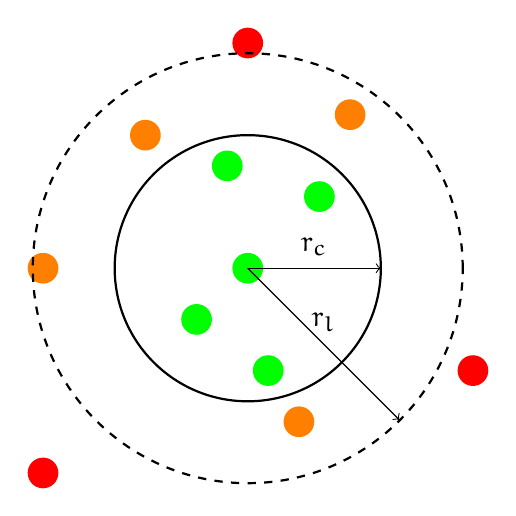
\begin{tikzpicture}[scale=1.3, transform shape]
		%\draw[gray,step=1] (-2,-2) grid (2,2);
		\fill[fill=green] (0,0) circle (0.15);
		\fill[fill=green] (-0.2,1) circle (0.15);
		\fill[fill=green] (-0.5,-0.5) circle (0.15);
		\fill[fill=green] (0.2,-1) circle (0.15);
		\fill[fill=green] (0.7,0.7) circle (0.15);
		\fill[fill=orange] (1,1.5) circle (0.15);
		\fill[fill=orange] (-1,1.3) circle (0.15);
		\fill[fill=orange] (-2,0) circle (0.15);
		\fill[fill=orange] (0.5,-1.5) circle (0.15);
		\fill[fill=red] (2.2,-1) circle (0.15);
		\fill[fill=red] (0,2.2) circle (0.15);
		\fill[fill=red] (-2,-2) circle (0.15);
		\draw[thick] (0,0) circle (1.3);
		\draw[dashed,thick] (0,0) circle (2.1);
		\draw[->] (0,0) -- (1.3,0) node[midway,above] {\footnotesize $r_c$};
		\draw[->] (0,0) -- (1.48, -1.48) node[midway,above] {\footnotesize $r_l$};
	\end{tikzpicture}
\end{document}
	